\documentclass[a4paper, oneside]{article}
\usepackage[english, russian]{babel}

\usepackage{fontspec}
\setmainfont[
  Ligatures=TeX,
  Extension=.otf,
  BoldFont=cmunbx,
  ItalicFont=cmunti,
  BoldItalicFont=cmunbi,
]{cmunrm}
\usepackage{unicode-math}

\usepackage[bookmarks=false]{hyperref}
\hypersetup{pdfstartview={FitH},
            pdfauthor={Павел Соболев}}

\usepackage[lmargin=23mm]{geometry}

\usepackage[table]{xcolor}
\usepackage{booktabs}
\usepackage{caption}

\usepackage{graphicx}
\graphicspath{ {./figures/} }

\usepackage{sectsty}
\sectionfont{\centering}
\subsubsectionfont{\centering \vspace{-0.5em}\normalfont\itshape}

\newcommand{\npar}{\par\vspace{\baselineskip}}
\newcommand{\su}{\vspace{-0.5em}}
\newcommand{\sd}{\vspace{0.5em}}

\setlength{\parindent}{0pt}

\hypersetup{pdftitle={Астрофизическая практика: отчет по третьей работе}}

\begin{document}

\section*{Работа №3: Фотоэлектрическая фотометрия \\ звезд скопления Плеяды}
\subsubsection*{Выполнил: Павел Соболев}

\vspace{3em}

\subsection*{Задачи}

\begin{itemize}
  \setlength\itemsep{-0.1em}
  \item Используя моделируемые с помощью компьютера телескоп и фотометр, измерить видимые B, V звездные величины;
  \item Построить диаграмму Герцшпрунга-Рессела для скопления (V vs (B\,-V));
  \item Определить расстояние до Плеяд.
\end{itemize}

\subsection*{Ход выполнения и результаты}

В ходе работы с виртуальным телескопом и фотометром были получены следующие данные:

\begin{table}[h]
  \centering
  \caption{Видимые звездные величины в фильтрах B и V (часть 1)}
  \begin{tabular}{cccccc}
    \toprule
    Звезда &
    Прямое восхождение &
    Склонение &
    B &
    V &
    B\,-V \\
    \midrule
    1 & 3$^h$ 41$^m$ 05$^s$ & 24$^\circ$ 05$'$ 11$''$ & 13.311 & 12.530 & 0.781 \\
    \arrayrulecolor{black!40}
    \midrule
    2 & 3$^h$ 42$^m$ 15$^s$ & 24$^\circ$ 19$'$ 57$''$ & 4.201 & 4.310 & -0.109 \\
    \midrule
    3 & 3$^h$ 42$^m$ 33$^s$ & 24$^\circ$ 18$'$ 55$''$ & 8.948 & 8.602 & 0.346 \\
    \midrule
    4 & 3$^h$ 42$^m$ 41$^s$ & 24$^\circ$ 28$'$ 22$''$ & 10.246 & 9.700 & 0.546 \\
    \midrule
    5 & 3$^h$ 43$^m$ 08$^s$ & 24$^\circ$ 42$'$ 47$''$ & 13.060 & 12.049 & 1.011 \\
    \midrule
    6 & 3$^h$ 43$^m$ 08$^s$ & 25$^\circ$ 00$'$ 46$''$ & 15.343 & 14.337 & 1.006 \\
    \midrule
    7 & 3$^h$ 43$^m$ 39$^s$ & 23$^\circ$ 28$'$ 58$''$ & 8.472 & 8.110 & 0.362 \\
    \midrule
    8 & 3$^h$ 43$^m$ 42$^s$ & 23$^\circ$ 20$'$ 34$''$ & 13.009 & 12.022 & 0.987 \\
    \midrule
    9 & 3$^h$ 43$^m$ 56$^s$ & 23$^\circ$ 25$'$ 46$''$ & 11.162 & 10.520 & 0.642 \\
    \midrule
    10 & 3$^h$ 44$^m$ 03$^s$ & 24$^\circ$ 25$'$ 54$''$ & 6.820 & 6.798 & 0.022 \\
    \midrule
    11 & 3$^h$ 44$^m$ 11$^s$ & 24$^\circ$ 07$'$ 23$''$ & 9.932 & 9.458 & 0.474 \\
    \midrule
    12 & 3$^h$ 44$^m$ 19$^s$ & 24$^\circ$ 14$'$ 16$''$ & 13.750 & 12.631 & 1.119 \\
    \midrule
    13 & 3$^h$ 44$^m$ 27$^s$ & 23$^\circ$ 57$'$ 57$''$ & 2.780 & 2.870 & -0.09 \\
    \midrule
    14 & 3$^h$ 44$^m$ 39$^s$ & 23$^\circ$ 27$'$ 17$''$ & 8.951 & 7.718 & 1.233 \\
    \midrule
    15 & 3$^h$ 44$^m$ 39$^s$ & 24$^\circ$ 34$'$ 47$''$ & 16.988 & 16.402 & 0.586 \\
    \midrule
    16 & 3$^h$ 44$^m$ 45$^s$ & 23$^\circ$ 24$'$ 52$''$ & 9.956 & 8.801 & 1.155 \\
    \midrule
    17 & 3$^h$ 45$^m$ 09$^s$ & 24$^\circ$ 50$'$ 59$''$ & 8.154 & 6.459 & 1.695 \\
    \midrule
    18 & 3$^h$ 45$^m$ 27$^s$ & 23$^\circ$ 17$'$ 57$''$ & 5.379 & 5.451 & -0.072 \\
    \midrule
    19 & 3$^h$ 45$^m$ 28$^s$ & 23$^\circ$ 53$'$ 41$''$ & 10.586 & 10.022 & 0.564 \\
    \arrayrulecolor{black}
    \bottomrule
  \end{tabular}
\end{table}

\newpage

\begin{table}[h]
  \centering
  \caption{Видимые звездные величины в фильтрах B и V (часть 2)}
  \begin{tabular}{cccccc}
    \toprule
    Звезда &
    Прямое восхождение &
    Склонение &
    B &
    V &
    B\,-V \\
    \midrule
    20 & 3$^h$ 45$^m$ 33$^s$ & 24$^\circ$ 12$'$ 59$''$ & 7.060 & 6.946 & 0.114 \\
    \arrayrulecolor{black!40}
    \midrule
    21 & 3$^h$ 46$^m$ 26$^s$ & 23$^\circ$ 41$'$ 11$''$ & 12.128 & 11.344 & 0.784 \\
    \midrule
    22 & 3$^h$ 46$^m$ 26$^s$ & 23$^\circ$ 49$'$ 58$''$ & 16.851 & 15.703 & 1.148 \\
    \midrule
    23 & 3$^h$ 46$^m$ 57$^s$ & 24$^\circ$ 04$'$ 51$''$ & 9.340 & 9.171 & 0.169 \\
    \midrule
    24 & 3$^h$ 47$^m$ 29$^s$ & 24$^\circ$ 20$'$ 34$''$ & 7.550 & 7.420 & 0.13 \\
    \arrayrulecolor{black}
    \bottomrule
  \end{tabular}
\end{table}

Построенная на основе этих данных диаграмма Герцшпрунга-Рессела выглядит так:

\begin{figure}[h]
  \centering
  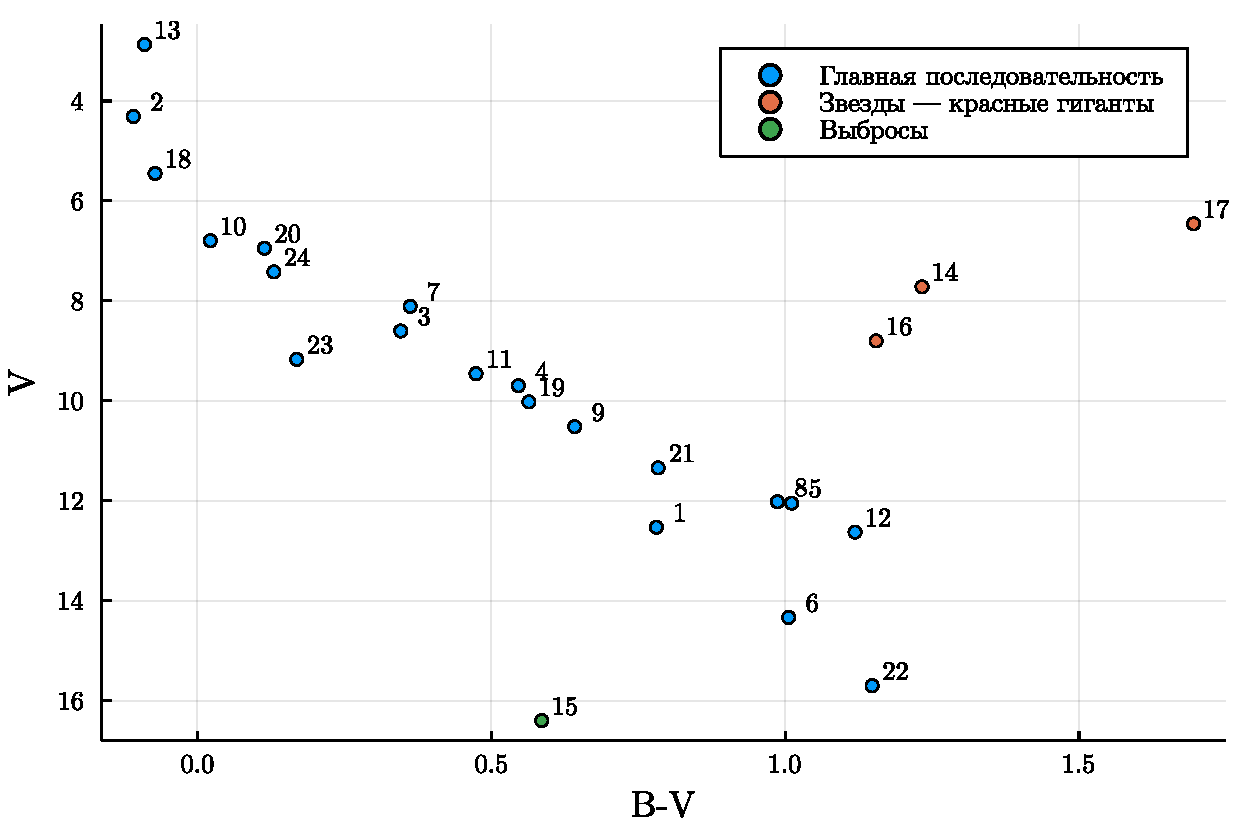
\includegraphics[scale=0.5]{diagram1}
  \caption{Диаграмма Герцшпрунга-Рессела}
\end{figure}

\newpage

Имеются следующие данные для абсолютных звездных величин:

\begin{table}[h]
  \centering
  \caption{Абсолютные звездные величины в зависимости от показателя цвета}
  \begin{tabular}{ccc}
    \toprule
    M &
    B\,-V &
    Класс \\
    \midrule
    -5.8 & -0.35 & O5 \\
    \arrayrulecolor{black!40}
    \midrule
    -4.1 & -0.31 & B0 \\
    \midrule
    -1.1 & -0.16 & B5 \\
    \midrule
    -0.7 & 0.0 & A0 \\
    \midrule
    2.0 & 0.13 & A5 \\
    \midrule
    2.6 & 0.27 & F0 \\
    \midrule
    3.4 & 0.42 & F5 \\
    \midrule
    4.4 & 0.58 & G0 \\
    \midrule
    5.1 & 0.70 & G5 \\
    \midrule
    5.9 & 0.89 & K0 \\
    \midrule
    7.3 & 1.18 & K5 \\
    \midrule
    9.0 & 1.45 & M0 \\
    \midrule
    11.8 & 1.63 & M5 \\
    \midrule
    16.0 & 1.80 & M8 \\
    \arrayrulecolor{black}
    \bottomrule
  \end{tabular}
\end{table}

Добавив эти данные на диаграмму Герцшпрунга-Рессела выше; убрав из измеренных данных звезды, не лежащие на главной последовательности; вписав в обе выборки полиномы третьей степени и вычислив разницу между ними, получаем следующий график:

\newpage

\begin{figure}[h]
  \centering
  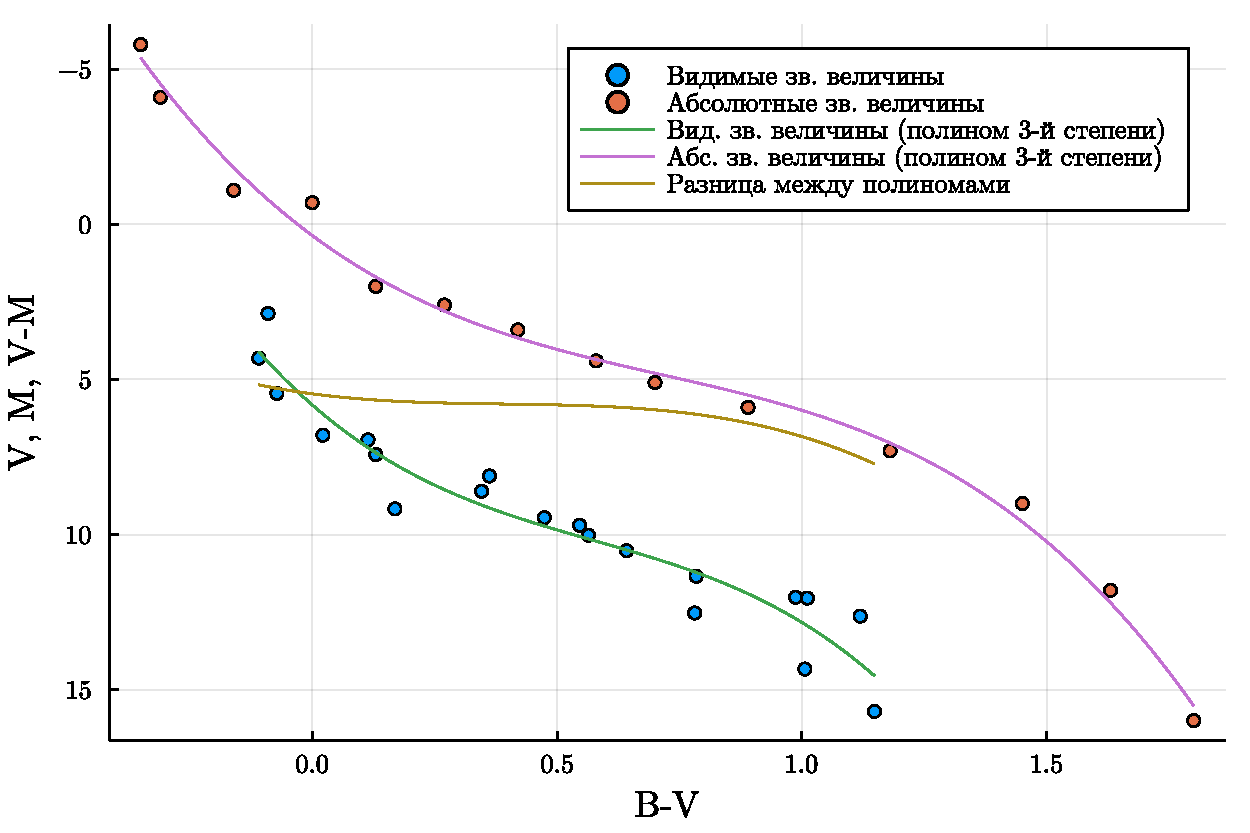
\includegraphics[scale=0.5]{diagram2}
  \caption{Разница между абсолютными и видимыми зв. величинами}
\end{figure}

Значение модуля разности (медианы $\pm$ межквартильного размаха разницы полиномов на области определения видимых звездных величин) равно $ 5.83 \pm 0.51 ^m $. \npar

Согласно

\su
$$
\lg{D} = (m - M + 5) / 5,
$$
\su

расстояние до скопления Плеяды равно $ 146.0 \pm 35.0 $ пк.

\end{document}